\documentclass{article}

\usepackage{graphicx}
\usepackage{tikz}
\usepackage{tikzsymbols}
\usetikzlibrary{calc,patterns,shapes.geometric}
\pagestyle{empty}
\usepackage[margin=0pt]{geometry}
\geometry{papersize={14in,12in}}

\def\centerarc[#1](#2)(#3:#4:#5){\draw[#1] ($(#2)+({#5*cos(#3)},{#5*sin(#3)})$) arc (#3:#4:#5);}

\begin{document}
	\begin{figure}
		\centering
		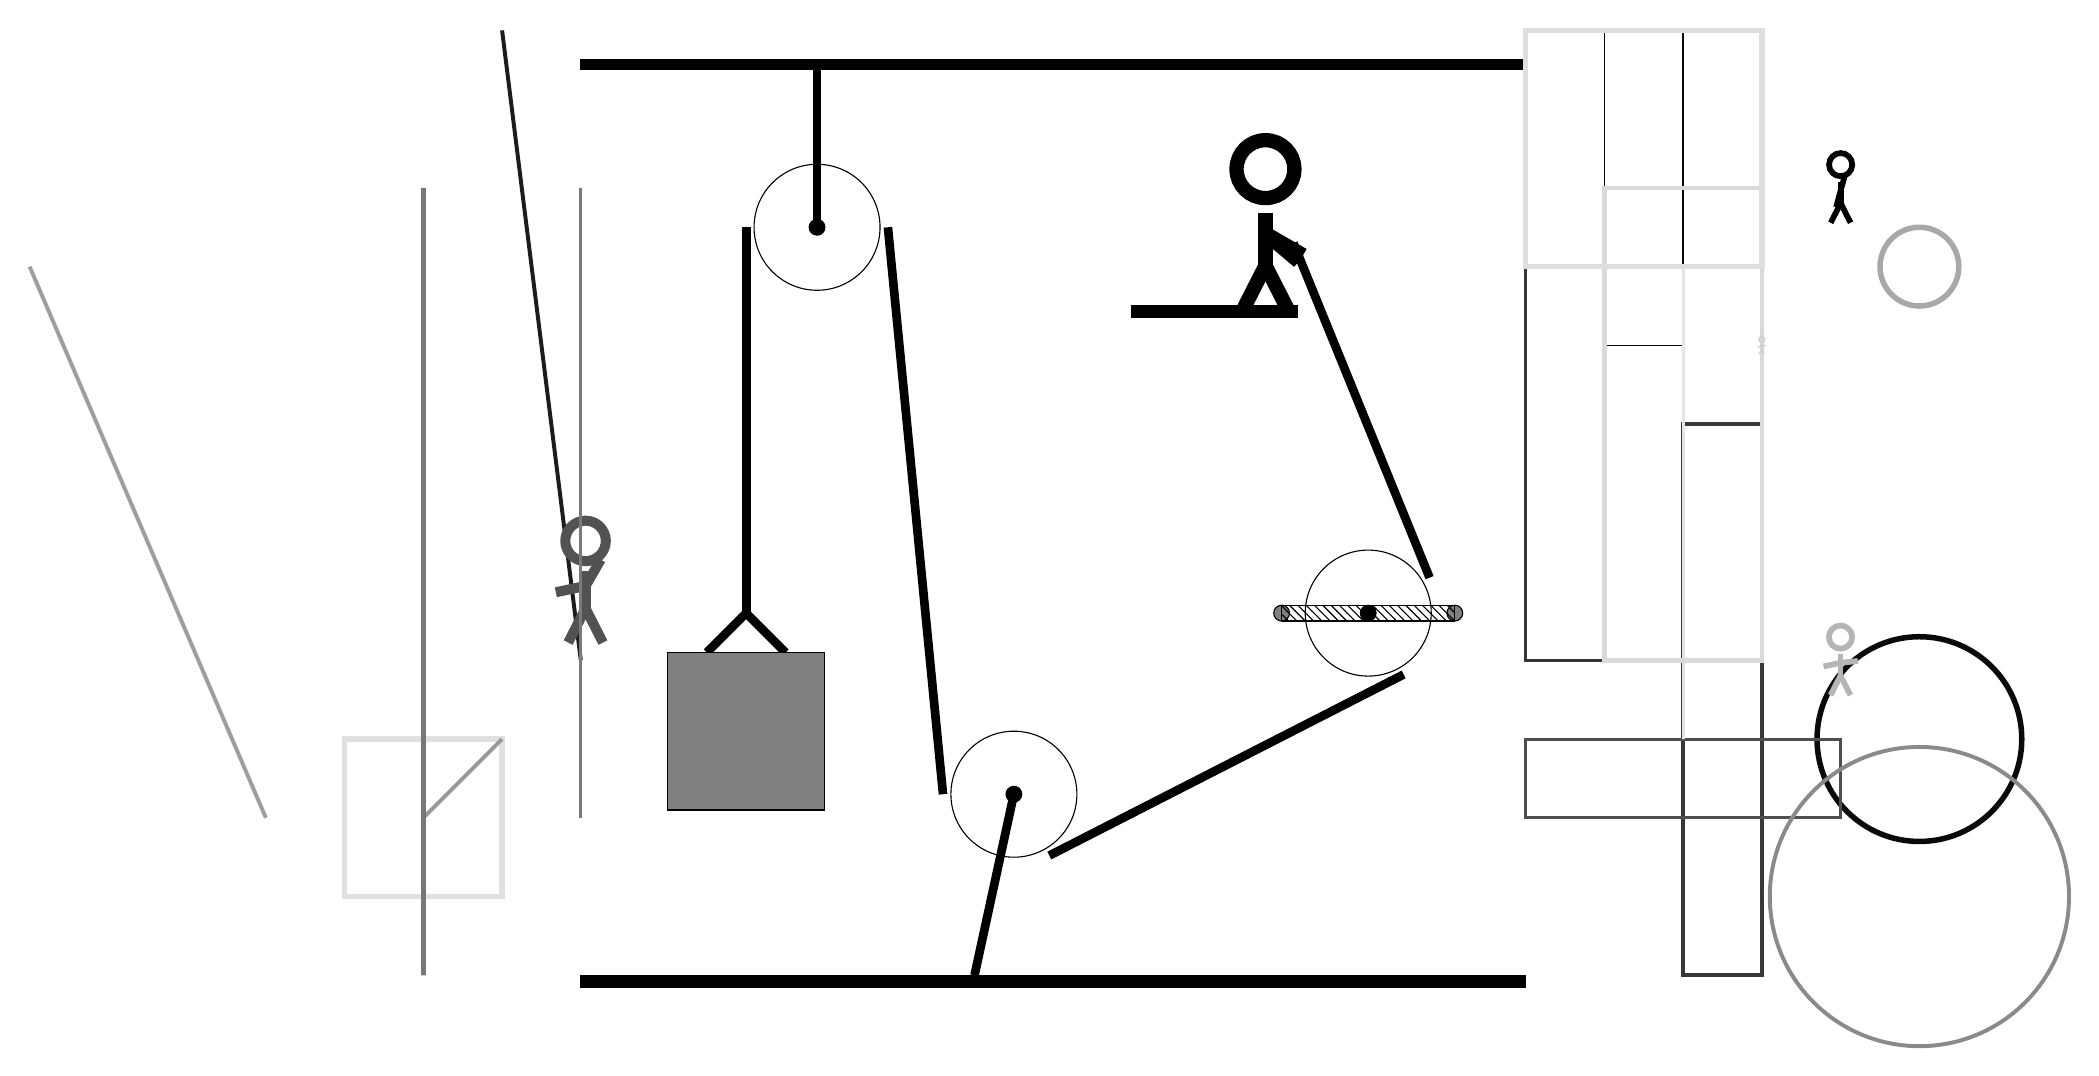
\begin{tikzpicture}
			%%%%% START %%%%%
			
			\draw[fill=black] (-2, 11.5) rectangle (10, 11.625);
			
			\draw (1, 9.5) circle (0.8);
			\draw[fill=black] (1, 9.5) circle (0.1);
			\draw[line width=1.1mm] (1, 11.5) -- (1, 9.5);
			
			\draw (3.5, 2.3) circle (0.8);
			\draw[fill=black] (3.5, 2.3) circle (0.1);
			\draw[line width=1.1mm] (3.5, 2.3) -- (3.0, 0);
			
			\draw[fill=white](8, 4.6) circle (0.8);
			\draw[fill=black] (8, 4.6) circle (0.1);
			\draw[fill=black!50] (9.1, 4.6) circle (0.1);
			\draw[fill=black!50] (6.9, 4.6) circle (0.1);
			\draw[pattern=north west lines, pattern color=black] (6.9, 4.7) rectangle (9.1, 4.5);
			
			\draw [line width=0.7mm, color=black!34](15, 9) circle (0.5);
			
			\draw[line width=0.5mm, color=black!78] (12, 7) rectangle (13, 0);
			\draw[line width=0.5mm, color=black!89](-3, 12) -- (-2, 4);
			\draw [line width=0.7mm, color=black!96](15, 3) circle (1.3);
			
			\draw[line width=0.4mm, color=black!79] (10, 4) rectangle (13, 9);
			\draw[line width=0.2mm, color=black!97] (11, 12) rectangle (12, 8);
			
			\draw[line width=0.4mm, color=black!69] (10, 2) rectangle (14, 3);
			
			\draw[line width=0.4mm, color=black!10] (12, 3) rectangle (12, 9);
			\draw[line width=0.6mm, color=black!15] (11, 10) rectangle (13, 4);
			
			\draw [line width=0.5mm, color=black!46](15, 1) circle (1.9);
			\draw[line width=0.7mm, color=black!12] (-3, 1) rectangle (-5, 3);
			\draw[line width=0.5mm, color=black!40](-3, 3) -- (-4, 2);
			\node[line width=0.4mm, color=black!68] at (-2, 5) {\Strichmaxerl[7][12][60]};
			\node[line width=0.7mm, color=black!29] at (14, 4) {\Strichmaxerl[4][12][6]};
			\node[line width=0.2mm, color=black!19] at (13, 8) {\Strichmaxerl[1][16][7]};
			\draw[line width=0.7mm, color=black!13] (10, 9) rectangle (13, 12);
			\draw[line width=0.5mm, color=black!38](-6, 2) -- (-9, 9);
			
			\node[line width=0.4mm, color=black!100] at (14, 10) {\Strichmaxerl[4][75][74]};
			\draw[line width=0.7mm, color=black!53] (-4, 0) rectangle (-4, 10);
			\draw[line width=0.4mm, color=black!52] (-2, 2) rectangle (-2, 10);
			
			\draw[line width=1.1mm](-0.4, 4.1) --  (0.1, 4.6) -- (0.6, 4.1);
			\draw[fill=black!50] (-0.9, 4.1) rectangle (1.1, 2.1);
			
			\draw[line width=1.1mm](0.1, 9.5) -- (0.1, 4.6);
			\centerarc[line width=1.1mm](1, 9.5)(180:0:0.9)
			\draw[line width=1.1mm](1.9, 9.5) -- (2.6, 2.3);
			\centerarc[line width=1.1mm](3.5, 2.3)(180:300:0.9);
			\draw[line width=1.1mm](3.95, 1.5206) -- (8.45, 3.8206);
			\centerarc[line width=1.1mm](8, 4.6)(300:390:0.9);
			\draw[line width=1.1mm](8.7794, 5.05) -- (7.05, 9.3);
			
			\node at (6.75, 9.5) {\Strichmaxerl[10][-220][-30]};
			\draw[fill=black] (5, 8.5) rectangle (7.1, 8.35);
			
			\draw[fill=black] (-2, 0) rectangle (10, -0.15);
			
			%%%%% END %%%%%
		\end{tikzpicture}
	\end{figure}	
\end{document}